\chapter{使用此模板}

\section{自动生成}
何为自动生成?

此模板的编写完全遵守《广东工业大学本科生毕业设计(论文)》的要求。你只需要用上以下会提到的一些注意要点,同时学习简单使用\TeX{}Maker或其他\TeX{}编辑器,编写好\TeX{}文件,加载本模板,并且运行批处理命令或自动运行脚本,成功编译后,你就能得到一份格式正确的论文。所有你所需要努力的就是写一个好的论文内容。免除格式的烦恼。关于编译,详细请看\ref{sec:compile}节。

\section{封面}
直接修改Cover.tex即可。详情看\ref{sec:cover}节。

\section{摘要}
模板已经设定好了摘要的环境,直接填入摘要文字,及关键字文字即可。
\begin{lstlisting}
\begin{cabstract}%`中文摘要`
\end{cabstract}
\ckeywords{`中文关键词`}
\begin{eabstract} %abstract
\end{cabstract}
\ekeywords{keywords}
\end{lstlisting}

\section{目录}
目录环境已经在模板内定义,直接使用\verb|\tableofcontents|命令即可。

\section{正文}
正文的文字书写环境已经模板内清楚定义,直接书写即可。换行的时候要注意,在\TeX{}源文件中,换行需要用到命令\verb|\\|、\verb|\par|或换两行(即使用两次回车键)。

\subsection{标题}
正文标题按级填写,不建议超过三级。
\begin{lstlisting}[language=TeX]
\chapter{`章标题`}
\section{`节标题`}
\subsection{`条标题`}
\end{lstlisting}

\subsection{字号及字符}
字符的设定及使用,见\ref{sec:fontsize}节;字号的设定及使用,见\ref{sec:font}节。

\subsection{特殊字符}
一些特殊符号需要用\TeX{}命令来表示,如\tabref{char}。\TeX{}Maker有直接生成数字符号的功能,方便大家使用。
\begin{table}[htbp]
\begin{center}
\caption{特殊字符输入}
\label{tab:char}
\begin{tabularx}{\linewidth}{Z|Z|Z|Z|Z|Z|Z|Z|Z|Z} \toprule
输入 & \verb|\#| & \verb|\$| & \verb|\%| & \verb|\&| & \verb|\{| & \verb|\}| & \verb|\_| & \verb|\^{}| & \verb|\~{}| \\\cline{1-10}
显示 & \# &	\$ & \% & \& & \{ & \} & \_	& \^{} & \~{} \\\cline{1-10}
输入 & \multicolumn{2}{Z|}{\verb|\textless|} & \multicolumn{2}{Z|}{\verb|\textgreater|} & \multicolumn{2}{Z|}{\verb|\textbar|} & \multicolumn{3}{Z}{\verb|\textbackslash|} \\\cline{1-10}
显示 & \multicolumn{2}{Z|}{\textless} & \multicolumn{2}{Z|}{\textgreater} & \multicolumn{2}{Z|}{\textbar} & \multicolumn{3}{Z}{\textbackslash} \\\bottomrule
\end{tabularx}
\end{center}
\end{table}

\section{插入表格}
此节介绍表格的画法。从简单的三线表,到复杂的内嵌表格。当然,你也直接可以用\TeX{}Maker画出你所需要的表格。根据《手册》中的规定,不介绍跨页表格的画法,需要跨页表格,可以通过分表格的方法。

\subsection{三线表}
表格的画法可以直接表现为线条的组合。如\tabref{tabexample1},仿制自《手册》24页的表3.3。

\begin{table}[htbp]
\begin{center}
%\caption{压降损失计算结果}
\Ucaption{压降损失计算结果}{Pa}
\label{tab:tabexample1}
\begin{tabularx}{\linewidth}{ZZZ}\toprule
换热器 & 热边压降损失 & 冷边压降损失\\\midrule
初级 & 2974.37 & 2931.52\\
次级 & 2924.65 & 3789.76\\\bottomrule
\end{tabularx}
\end{center}
\end{table}

代码如下:

\begin{lstlisting}[language=TeX]
\begin{table}[htbp]
\begin{center}
\caption{压降损失计算结果}\raisebox{0.75em}[-1.2em]{\hspace*{0.5\linewidth}\heiti \bfseries Pa}
\label{tab:tabexample1}
\begin{tabularx}{\linewidth}{ZZZ}\toprule
`换热器` & `热边压降损失` & `冷边压降损失`\\\midrule
`初级` & 2974.37 & 2931.52\\
`次级` & 2924.65 & 3789.76\\\bottomrule
\end{tabularx}
\end{center}
\end{table}
\end{lstlisting}

假如制作简单的表格可以直接用此模板。在table的浮动环境下,设定一个居中的环境,在居中环境里面添加标题\textbackslash caption。加入引用标签\textbackslash label,这样就可以随时在正文中使用\textbackslash tabref命令引用相关表格。接下来就是画表,使用四周(上下左右)居中的环境Z,表格宽度为版心宽度\textbackslash linewidth。\textbackslash toprule为顶边的线,midrule为中间的线,bottomrule为底边线。

需要注意的是,由于\tabref{tabexample1}比较特殊,在标题后面有一个标记压强单位Pa,所以用了\textbackslash raisebox命令建立了一个向上移动0.75个字符,深度(即字体间距)为-1.2个字符的上升盒子来装“Pa”。这个并非必须,这个功能类似于Word里面的文本框功能,当你想放置一些无序的内容时,可以使用它。

\subsection{复杂表格}
复杂表格\tabref{tabexample2},仿制自《手册》24页的表2.1。

\begin{table}[htbp]
\begin{center}
\caption{方法——干扰抑制结果}
\label{tab:tabexample2}
\begin{tabularx}{\linewidth}{Z|Z|Z|Z|Z} \toprule
干扰类型 & 目标信号 & 阵元数 & 干扰采样指数 & SINR(dB) \\\cline{1-5}
\multirow{4}*{第一类干扰} & \multirow{2}*{信号1} & 8 & -- & 30.58 \\\cline{3-5} 
& & 4 & -- & 21.16 \\\cline{2-5} 
& \multirow{2}*{信号4} & 8 & -- & 38.28 \\\cline{3-5} 
& & 4 & -- & 19.41 \\\hline
\multirow{3}*{第二类干扰} & \multirow{3}*{信号4} & \multirow{2}*{8} & 30 & 4.69 \\\cline{4-5} 
& & & 19 & 4.83 \\\cline{3-5} 
& & 4 & 30 & -4.42 \\\bottomrule
\end{tabularx}
\end{center}
\end{table}

代码如下:

\begin{lstlisting}[language=TeX]
\begin{table}[htbp]
\begin{center}
\caption{`方法——干扰抑制结果`}
\label{tab:tabexample2}
\begin{tabularx}{\linewidth}{Z|Z|Z|Z|Z} \toprule
`干扰类型` & `目标信号` & `阵元数` & `干扰采样指数` & SINR(dB) \\\cline{1-5}
\multirow{4}*{`第一类干扰`} & \multirow{2}*{`信号1`} & 8 & -- & 30.58 \\\cline{3-5} 
& & 4 & -- & 21.16 \\\cline{2-5} 
& \multirow{2}*{`信号4`} & 8 & -- & 38.28 \\\cline{3-5} 
& & 4 & -- & 19.41 \\\hline
\multirow{3}*{`第二类干扰`} & \multirow{3}*{`信号4`} & \multirow{2}*{8} & 30 & 4.69 \\\cline{4-5} 
& & & 19 & 4.83 \\\cline{3-5} 
& & 4 & 30 & -4.42 \\\bottomrule
\end{tabularx}
\end{center}
\end{table}
\end{lstlisting}

表格假如需要全局的竖线,可以直接在Z环境后加上竖线如\{Z\textbar Z\textbar Z\}。由于有一些格需要跨行合并,所以需要\textbackslash multirow命令,multirow\{4\}*\{第一类干扰\}代表者跨4行,×表示数据自然高度,\{\}里为内容。\textbackslash cline命令可以设置划线的列数,例如\textbackslash cline{3-5}为从第三列画到第5列。\textbackslash hline可以画出与表格宽度相等的线,类似于\textbackslash midrule。

要注意,被合并行是从上往下数,即第一行合并了下面的二、三、四行,所以二、三、四行的第一个空个的内容皆为空。

介绍另外一种复杂表格,需要用到列合并。复杂表格\tabref{tabexample3},仿制自《手册》24页的表3.1(摘其中几行作为示例)。

\begin{table}[htbp]
\begin{center}
\caption{各分组lgB$_{i}$值}
\label{tab:tabexample3}
\begin{tabularx}{\linewidth}{ZZZZZ} \toprule
\multirow{2}*{序号} & \multicolumn{2}{|c|}{\textit{T}=1500K} & \multicolumn{2}{c}{\textit{T}=2000K} \\\cline{2-5}
 & \multicolumn{1}{|Z}{组分} & \multicolumn{1}{|Z|}{lgB$_{i}$} & 组分 & \multicolumn{1}{c}{lgB$_{i}$} \\\midrule
1 & O$_{2}$$^{+}$ & 5.26 & HO$_{2}$ & 6.43 \\
6 & OH & 3.29 & OH & 5.91 \\
10 & H$_{2}$O$_{2}$ & 1.62 & CO$_{2}$$^{+}$ & 3.76 \\
12 & HCO$^{*}$ & -0.47 & HCO$^{*}$ & 0.24 \\\bottomrule
\multicolumn{5}{l}{\xiaowu 注:“+”表示重要部分,“*”表示冗余组分。} \\
\end{tabularx}
\end{center}
\end{table}

代码如下:

\begin{lstlisting}[language=TeX]
\begin{table}[htbp]
\begin{center}
\caption{`各分组lgB$_{i}$值`}
\label{tab:tabexample3}
\begin{tabularx}{\linewidth}{ZZZZZ} \cline{1-5}
\multirow{2}*{`序号`} & \multicolumn{2}{|c|}{\textit{T}=1500K} & \multicolumn{2}{c}{\textit{T}=2000K} \\\cline{2-5}
 & \multicolumn{1}{|Z}{`组分`} & \multicolumn{1}{|Z|}{lgB$_{i}$} & `组分` & \multicolumn{1}{c}{lgB$_{i}$} \\\cline{1-5}
1 & O$_{2}$$^{+}$ & 5.26 & HO$_{2}$ & 6.43 \\
6 & OH & 3.29 & OH & 5.91 \\
10 & H$_{2}$O$_{2}$ & 1.62 & CO$_{2}$$^{+}$ & 3.76 \\
12 & HCO^{*} & -0.47 & HCO$^{*}$ & 0.24 \\\cline{1-5}
\multicolumn{5}{l}{\xiaowu `注:“+”表示重要部分,“*”表示冗余组分。`} \\
\end{tabularx}
\end{center}
\end{table}
\end{lstlisting}

\textbackslash multicolumn命令是列合并。\textbackslash multicolumn\{2\}\{\textbar c\textbar\}\{\textbackslash textit\{T\}=1500K\}表达的意思是合并2列表格,合并后的表格内容居中并且两边生成竖边框,内容为斜体的T=1500K。\textbackslash multicolumn命令运作方式与\textbackslash multicolumn有所不同,如第一行,由于\textbackslash multicolumn命令的作用,该行仅有三个空需要填入内容。假如需要行列合并的话,可以使用\textbackslash multicolumn\{行数\}\{对齐\}\{\textbackslash multirow\{列数\}*\{内容\}\}

关于脚注,由于《手册》中要求脚注前要加上注,\textbackslash footnote命令无法达到效果,所以建议用\textbackslash multicolumn命令生成一个左对齐的无边框单行表格,然后直接输入相关文字即可。

另外,\verb|\^{}|为上标,\verb|\_{}|为下标。可以直接用\TeX{}Maker生成。

\subsection{子表格}
子表格经常用于表格之间的比对。如,\tabref{parallel1}、\tabref{parallel2}

\begin{table}[htbp]
\noindent\begin{minipage}{0.45\textwidth}
\centering
\caption{第一个并排子表格}
\label{tab:parallel1}
\begin{tabularx}{0.45\textwidth}{Z|Z}
\toprule
111 & 222 \\\midrule
222 & 333 \\\bottomrule
\end{tabularx}
\end{minipage}
\begin{minipage}{0.45\textwidth}
\centering
\caption{第二个并排子表格}
\label{tab:parallel2}
\begin{tabularx}{0.45\textwidth}{Z|Z}
\toprule
111 & 222 \\\midrule
222 & 333 \\\bottomrule
\end{tabularx}
\end{minipage}
\end{table}

代码如下:

\begin{lstlisting}[language=TeX]
\begin{table}[htbp]
\noindent\begin{minipage}{0.45\linewidth}
\centering
\caption{`第一个并排子表格`}
\label{tab:parallel1}
\begin{tabularx}{0.45\linewidth}{Z|Z}\toprule
111 & 222 \\\midrule
222 & 333 \\\bottomrule
\end{tabularx}
\end{minipage}
\begin{minipage}{0.45\linewidth}
\centering
\caption{`第二个并排子表格`}
\label{tab:parallel2}
\begin{tabularx}{0.45\linewidth}{Z|Z}\toprule
111 & 222 \\\midrule
222 & 333 \\\bottomrule
\end{tabularx}
\end{minipage}
\end{table}
\end{lstlisting}

用小页环境minipage,把table环境分割成为两小块,每块为版心宽的0.45倍。

除了使用小页环境之外,我们也可以用子表格环境。如\tabref{subtable}。

\begin{table}[htbp]
\centering
\caption{并排子表格}
\label{tab:subtable}
\subfloat[第一个子表格]{
\begin{tabularx}{0.4\linewidth}{Z|Z}\toprule
111 & 222 \\\midrule
222 & 333 \\\bottomrule
\end{tabularx}}\hspace{0.15\linewidth}
\subfloat[第二个子表格]{
\begin{tabularx}{0.4\linewidth}{Z|Z}\toprule
111 & 222 \\\midrule
222 & 333 \\\bottomrule
\end{tabularx}}
\end{table}

代码如下:

\begin{lstlisting}[language=TeX]
\begin{table}[htbp]
\centering
\caption{`并排子表格`}
\label{tab:subtable}
\subfloat[`第一个子表格`]{
\begin{tabularx}{0.4\linewidth}{Z|Z}\toprule
111 & 222 \\\midrule
222 & 333 \\\bottomrule
\end{tabularx}}\hspace{0.15\linewidth}
\subfloat[`第二个子表格`]{
\begin{tabularx}{0.4\linewidth}{Z|Z}\toprule
111 & 222 \\\midrule
222 & 333 \\\bottomrule
\end{tabularx}}
\end{table}
\end{lstlisting}

由于《手册》中并未明确表明可以使用子表格,仅供大家参考。

\section{插图}
本章简单介绍一些在《手册》下适用的插图方法,假如需要了解更多,建议读一下《\LaTeXe 插图指南》\upcite{graphics}。

\subsection{单个图形}
\figref{figexample1}仿照《手册》的22页的图2.3。

\begin{figure}[htbp]
\begin{center}
{\rotatebox{90}{\hspace{13.5mm} \xiaowu 所有用户的平均误差比特率}}{\hspace{15mm}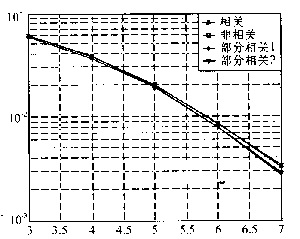
\includegraphics[height=65mm]{1.jpg}}{\hspace*{20mm}}
\end{center}
\vspace{-1.5em}
\hspace{-4em} {\xiaowu[0.75] 信噪比/dB}\\
{\centering {\xiaowu[0.75] \noindent 注:此图中的曲线对应关系与图2.1相同.}\\}
\caption{部分相干调解与相干和非相干调解平均误码性能的比较}
\label{fig:figexample1}
\end{figure}

代码如下:

\begin{lstlisting}[language=TeX]
\begin{figure}[htbp]
\begin{center}
{\rotatebox{90}{\hspace{13.5mm} \xiaowu `所有用户的平均误差比特率`}}{\hspace{15mm}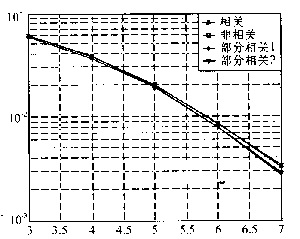
\includegraphics[height=65mm]{1.jpg}}{\hspace*{20mm}}
\end{center}
\vspace{-1.5em}
\hspace{-4em} {\xiaowu[0.75] `信噪比/dB`}\\
{\centering {\xiaowu[0.75] \noindent `注:此图中的曲线对应关系与图2.1相同.`}\\}
\caption{`部分相干调解与相干和非相干调解平均误码性能的比较`}
\label{fig:figexample1}
\end{figure}
\end{lstlisting}

主体部分是\textbackslash includegraphics[高度]\{图片\}。

另外,为了达到原图的效果,使用了\textbackslash rotatebox,旋转盒子的命令,把文字旋转90度至于图片左边。又通过用\textbackslash hspace\{\},水平间距命令及\textbackslash vspace\{\},垂直间距命令,把“信噪比/dB”放置于对齐于图片的左下角。同时使用\textbackslash centering命令把注解居中于图标题上方。以达到图2.3的效果。

字号的中括号内容表示行距设定。\LaTeX{}的行距设定在换字号大小的时候才会生效。为了使表格的注解能够比较紧凑,用0.75倍的行距比较适宜。

下\figref{figexample2}仿制《手册》22页的图3.1。

\begin{figure}[htbp]
\begin{center}
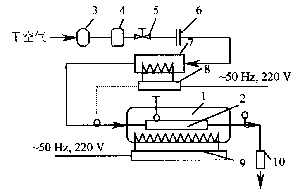
\includegraphics[height=50mm]{2.png}\\
{{\xiaowu[0.75]{1-太阳模拟器;2-单管及31个PCM容器;3-气泵;\\
4-干燥过滤器;5-手动调节阀;6-孔板流量计;\\
7-空气预热器;8,9-调功器;10-空气换热器。\\}}}
\end{center}
\caption{单管换热系统流程图}
\label{fig:figexample2}
\end{figure}

代码如下:

\begin{lstlisting}[language=TeX]
\begin{figure}[htbp]
\begin{center}
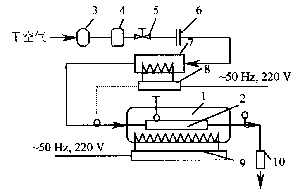
\includegraphics[height=50mm]{2.png}\\
{{\xiaowu[0.75]{`1-太阳模拟器;2-单管及31个PCM容器;3-气泵;`\\
`4-干燥过滤器;5-手动调节阀;6-孔板流量计;`\\
`7-空气预热器;8,9-调功器;10-空气换热器。`\\}}}
\end{center}
\caption{单管换热系统流程图}
\label{fig:figexample2}
\end{figure}
\end{lstlisting}

相较\figref{figexample1},\figref{figexample2}显得简单得多,我们的插图一般以这种为主。

\subsection{多个图形}
多个图形的编排与多个表格的编排基本相同,可以用小页minipage分割,或者使用subfigure子图片环境。

\figref{figexample3}展示的是《手册》23页的图2.5。

\begin{figure}[htbp]
\centering
\subfloat[分布符合1/f规律图]{%
\label{fig:subfig1}

\includegraphics[height=40.8mm]{3.png}}\hspace{4em}%
\subfloat[大小与色彩符合1/f规律图]{%
\label{fig:subfig2}
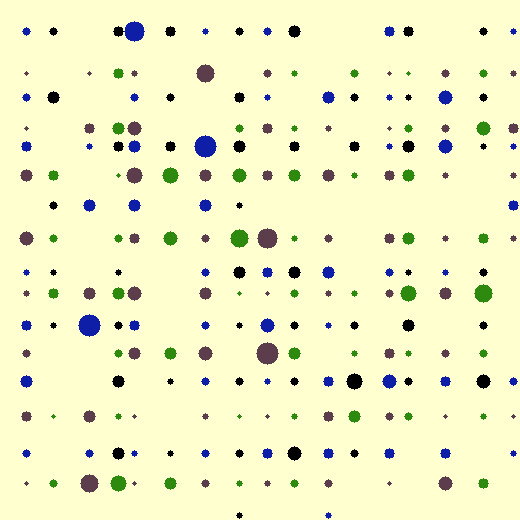
\includegraphics[height=38.4mm]{4.png}}\hspace{4em}
\subfloat[间距、大小与色彩均符合1/f规律图]{%
\label{fig:subfig3}

\includegraphics[height=41.7mm]{5.jpg}}
\caption{图案例}
\label{fig:figexample3}
\end{figure}

代码如下:

\begin{lstlisting}[language=TeX]
\begin{figure}[htbp]
\centering
\subfloat[`分布符合1/f规律图`]{%
\label{fig:subfig1}

\includegraphics[height=40.8mm]{3.png}}\hspace{4em}%
\subfloat[`大小与色彩符合1/f规律图`]{%
\label{fig:subfig2}
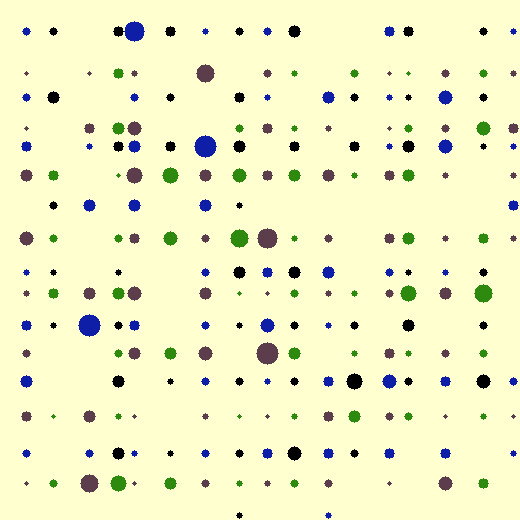
\includegraphics[height=38.4mm]{4.png}}\hspace{4em}
\subfloat[`间距、大小与色彩均符合1/f规律图`]{%
\label{fig:subfig3}

\includegraphics[height=41.7mm]{5.jpg}}
\caption{`图案例`}
\label{fig:figexample3}
\end{figure}
\end{lstlisting}

需要注意的是,图与图之间的间距,需要用水平间距命令进行调整。

\section{公式定理}
\TeX{}处理公式的能力非常强大,建议读取amsmath宏包的说明文档\upcite{amsmath}。下面举几个简单的例子,皆在公式环境equation中生成,对付不同的公式已经够了。其中的数学符号,可以在Web Equation网页中手写生成。

\begin{figure}[htbp]
\begin{center}
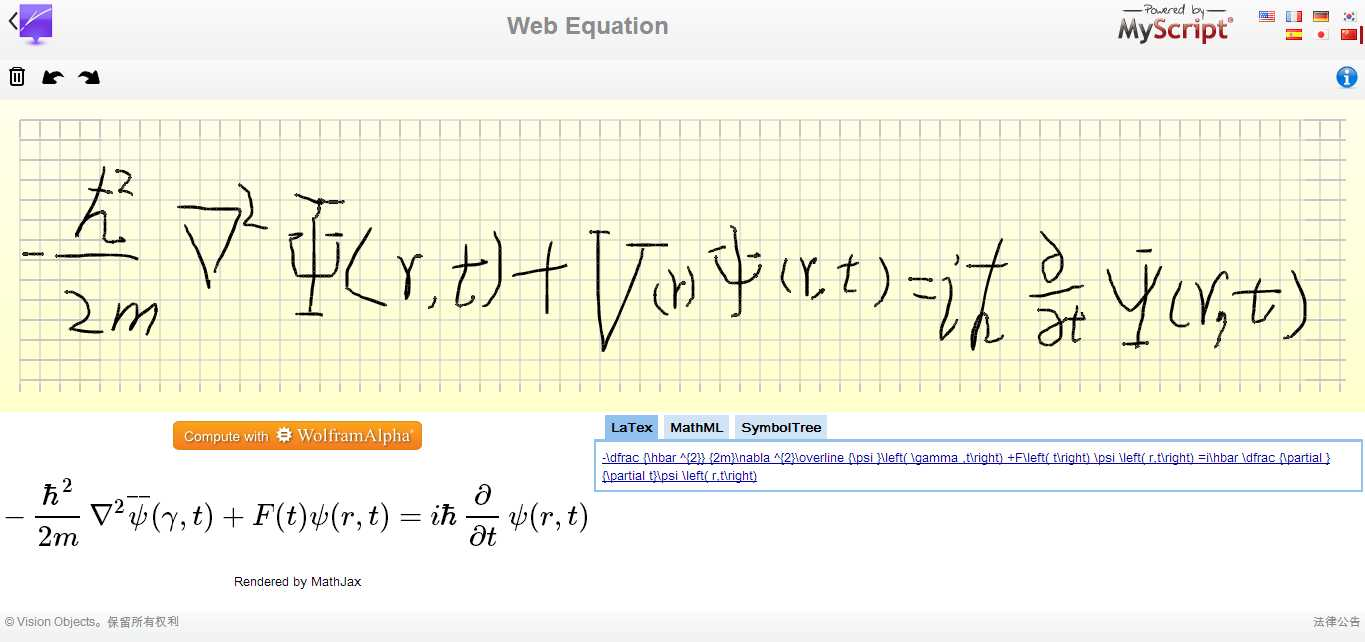
\includegraphics[width=0.9\linewidth]{wq.png}
\end{center}
\caption{用Web Equation生成\TeX{}公式代码}
\end{figure}

\subsection{单个公式}

\newcommand{\envert}[1]{\left\lvert#1\right\rvert} 
\begin{equation}\label{detK2}
\det\mathbf{K}(t=1,t_1,\dots,t_n)=\sum_{I\in\mathbf{n}}(-1)^{\envert{I}}
\prod_{i\in I}t_i\prod_{j\in I}(D_j+\lambda_jt_j)\det\mathbf{A}
^{(\lambda)}(\overline{I}|\overline{I})=0.
\end{equation} 

\begin{multline}%\tag{[b]} % 这个出现在索引中的
\int_a^b\biggl\{\int_a^b[f(x)^2g(y)^2+f(y)^2g(x)^2]
 -2f(x)g(x)f(y)g(y)\,dx\biggr\}\,dy \\
 =\int_a^b\biggl\{g(y)^2\int_a^bf^2+f(y)^2
  \int_a^b g^2-2f(y)g(y)\int_a^b fg\biggr\}\,dy
\end{multline}

\subsection{多列公式}

\begin{equation} 
\overrightarrow {p}_{i}\left( u\right) =\sum _{j=0}^{k}\overrightarrow {V}_{i}\Lambda _{i}\left( k;\overrightarrow {\beta }_{1},\ldots \overrightarrow {\beta }_{n};u\right)
\end{equation}

\begin{equation} 
\dfrac {\left| A\left( s\right) \right| ^{2}} {\left| A\left( O\right) \right| ^{2}}=\dfrac {\rho _{1}\rho _{2}} {\left( s+p_{1}\right) \left( s+\rho _{2}\right) }
\end{equation}

\section{代码高亮}
有些时候我们需要在论文中引入一段代码。
在模板中,统一使用\textbackslash listings宏包,并且设置了基本的内容格式。由于Lstlisting宏包对中文支持不太完善,可以设置中文逃逸,\textbackslash lstset\{escapeinside=\`{}\`{}\},用键盘数字符号键“1”左边的“倒引号”“\`{}”作为逃逸标记。但请注意,在Verilog语言中,左引号为特殊符号。

C语言示例:

\begin{lstlisting}[language=C]
#include <stdio.h>
main()
{printf("Hello World!\n"); %"`你好,世界`"
}
\end{lstlisting}

\section{参考文献}
参考文献可以用thebibliography环境生成,代码如下:

\begin{lstlisting}[language=TeX]
\begin{thebibliography}{}
\bibitem[`序号`]{`引用`} `文献信息`
\bibitem[1]{b1} Wikipedia. Linux[EB/OL]. http://zh.wikipedia.org/wiki/Linux,2013-5-20/2013-5-26. 
\end{thebibliography}
\end{lstlisting}

其中[]中填入文献前标号,缺省为数字排列,\{\}中为引用标签,例如\{r1\}则可在其他地方用指令\verb|\cite{r1}|引用标签上标可以使用\textbackslash textsuperscript命令,用法与\textbackslash cite一样。

\section{致谢}
致谢可以直接使用ack环境。直接输入文字即可。

\section{附录}
使用appxchp环境,在环境里使用\textbackslash appxtoc\{标题内容\}生成符合《手册》要求的附录。同时如需要生成图或表格的标题,使用\textbackslash appxfig(图) 和\textbackslash appxtab(表) 命令。引用标题的方法与正文相同。其他的操作与正文一样。

\section{编译}
\label{sec:compile}
好的,恭喜你,你终于写完了\TeX{}原文档了。是时候开始编译了。但在这之前,你还需要以下步骤:

1、创建一个空文件夹,名称如:gdutthesis

2、把thesis.tex、gdutthesis.cls、mygdut.sty、makepdf.bat、makefile三个文件放到你新建的文件夹里。

3、在这个新文件夹下建立两个新的空文件夹,data和figure。

4、把除thesis.tex以外的\TeX{}源文件放到Data下。记得在thesis.tex里用\textbackslash input命令加载它们。

5、把一切需要调用的图片都放在figure文件夹下面。

6、这个时候,可以开始编译了。

7、在命令行中,用cd命令定位到到你的\TeX{}源文件目录下,输入以下的代码,即可以编译thesis.tex文件了。\TeX{}文件需要经过三次编译才能正确显示效果\upcite{jmshouce}。 

\begin{lstlisting}[language=TeX]
xelatex thesis
xelatex thesis
xelatex thesis
\end{lstlisting}

8、最后祈祷一下吧,理论上不出错的话你就能得到一份比较不错的论文了。

9、补充一点,假如你觉得以上的步骤相当复杂,那么你可以直接在这份PDF文件的源文件夹下面操作。
